% System overview figure (Figure 1), drawn in TikZ. Panel (a): lf-013 inference loop; (b) route targets on a bend;
% (c) bend veto. Panels (b) and (c) are schematic. The camera thumbnail is a frame rendered in our local AlpaSim run
% (openai_golf/lead-candidate-2026-11-07/outputs/frames/9ad434ec99685d35-CAM_F0-1017000.jpg, public track assets).
\definecolor{pubF}{HTML}{E9EFF7}\definecolor{pubB}{HTML}{8DA2C0}
\definecolor{ourF}{HTML}{FCE8DC}\definecolor{ourB}{HTML}{E0662F}
\definecolor{headF}{HTML}{F5EFDA}\definecolor{headB}{HTML}{C4B37C}
\definecolor{simF}{HTML}{F3F3F1}\definecolor{simB}{HTML}{9B9A95}
\definecolor{inkC}{HTML}{3A3A3A}\definecolor{mutedC}{HTML}{6B6A66}
\definecolor{routeC}{HTML}{4A6FA5}\definecolor{grpF}{HTML}{FAFBFD}
\resizebox{\linewidth}{!}{%
\begin{tikzpicture}[x=1cm,y=1cm,font=\footnotesize,>=Latex,
  box/.style={rounded corners=2pt,align=center,inner sep=3pt},
  pub/.style={box,draw=pubB,fill=pubF},
  our/.style={box,draw=ourB,fill=ourF,line width=0.8pt},
  head/.style={box,draw=headB,fill=headF},
  sim/.style={box,draw=simB,fill=simF},
  arr/.style={->,line width=0.7pt,draw=inkC},
  lab/.style={font=\scriptsize,text=mutedC,align=center},
  ttl/.style={anchor=west,font=\small\bfseries}]

% ---------------------------------------------------------------- (a) inference loop
\node[ttl] at (-0.1,0.25) {(a) Policy and inference loop of \texttt{lf-013}};

% public checkpoint group
\draw[rounded corners=3pt,draw=pubB!70,fill=grpF] (2.35,-0.55) rectangle (8.95,-3.2);
\node[anchor=north west,font=\scriptsize\itshape,text=mutedC] at (2.4,-0.58)
  {Public Latent TransFuser checkpoint (py123d\_garage v0.2.0), unchanged};

% camera stack
\node[inner sep=0,draw=simB,line width=0.4pt] at (1.20,-1.62) {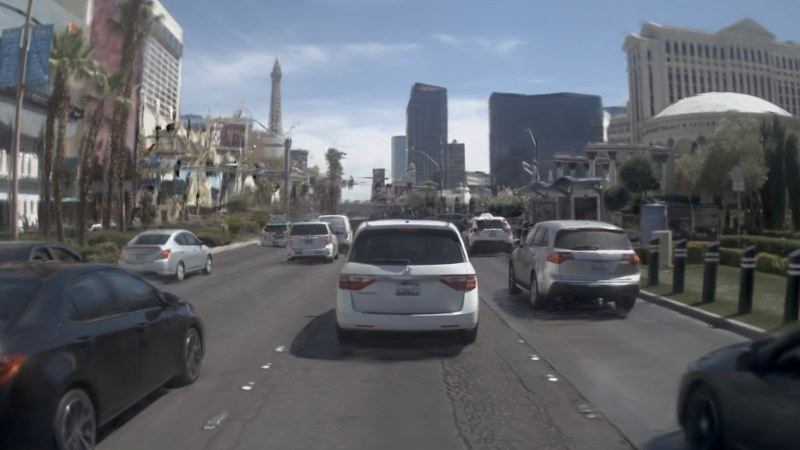
\includegraphics[width=1.9cm]{figures/front_camera_9ad434ec.jpg}};
\node[inner sep=0,draw=white,line width=0.8pt] (cam) at (1.05,-1.80) {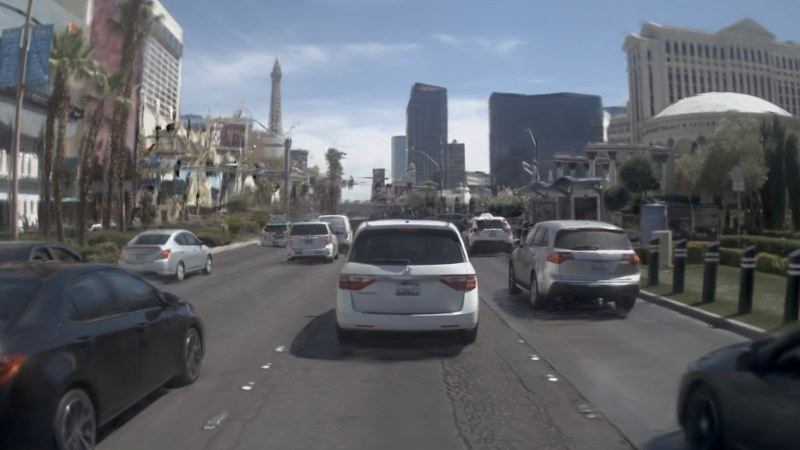
\includegraphics[width=1.9cm]{figures/front_camera_9ad434ec.jpg}};
\node[lab,anchor=south,text=inkC] at (1.13,-1.05) {\small Front camera};
\node[lab,anchor=north] at (1.05,-2.38) {\texttt{PCAM\_F0}: now, $-1$\,s\\352$\times$512};

% encoder, BEV, heads, planner
\node[trapezium,trapezium angle=70,shape border rotate=270,draw=pubB,fill=pubF,minimum height=1.25cm,
      minimum width=1.0cm,align=center,inner sep=1pt] (enc) at (3.25,-1.95) {Vision\\encoder};
\node[lab,anchor=north] at (3.25,-2.62) {ResNet-34};
\draw[pubB,fill=pubF] (4.35,-2.35) rectangle (5.15,-1.55);
\draw[pubB!80,step=0.16] (4.35,-2.35) grid (5.15,-1.55);
\node[lab,anchor=north] at (4.75,-2.4) {latent BEV};
\node[head,minimum width=2.9cm] (heads) at (7.15,-1.42) {Auxiliary heads\\[-1pt]{\scriptsize BEV road map $\cdot$ object boxes}};
\node[pub,minimum width=2.9cm] (plan) at (7.15,-2.5) {Flow-matching planner\\[-1pt]{\scriptsize waypoint flow, 8 steps, $T{=}0$}};

\draw[arr] (cam.east) -- (enc.west);
\draw[arr] (enc.east) -- (4.35,-1.95);
\draw[arr] (5.15,-1.95) -- (5.45,-1.95) |- (heads.west);
\draw[arr] (5.45,-1.95) |- (plan.west);

% inputs below the group
\node[our,text width=3.9cm] (route) at (4.55,-3.85) {Route targets 40/60/80\,m\\[-1pt]{\scriptsize along the route (ours, panel b)}};
\node[pub] (speed) at (8.05,-3.85) {Ego speed};
\coordinate (rin) at (6.75,-3.85);
\draw[arr] (route.east) -- (rin) -- (rin |- plan.south);
\draw[arr] (speed.north) -- (speed.north |- plan.south);

% outputs
\node[pub] (poses) at (9.95,-2.5) {64 poses\\[-1pt]{\scriptsize 0.1\,s apart, 6.4\,s}};
\node[our] (veto) at (11.85,-2.5) {Bend veto\\[-1pt]{\scriptsize ours, panel c}};
\node[sim] (simu) at (13.85,-2.5) {AlpaSim\\[-1pt]{\scriptsize controller}\\[-1pt]{\scriptsize + NuRec render}};
\draw[arr] (plan.east) -- (poses.west);
\draw[arr] (poses.east) -- (veto.west);
\draw[arr] (veto.east) -- (simu.west);
\draw[arr,dashed,draw=headB!90!black] (heads.east) -- (11.85,-1.42) -- (veto.north);
\node[lab,anchor=north] at (10.3,-1.47) {predicted road map,\\object boxes};

% closed loop
\draw[arr,draw=simB!90!black] (simu.north) -- (13.85,-0.25) -- (1.13,-0.25) -- (1.13,-0.7);
\node[lab,anchor=south] at (11.2,-0.25) {rendered frame, ego state, route};

% ---------------------------------------------------------------- (b) route targets
\begin{scope}[shift={(0,-9.25)}]
\node[ttl] at (-0.1,4.55) {(b) Route targets on a bend (every entry from \texttt{lf-009})};
% road band with edges
\draw[line width=19pt,draw=gray!45,line cap=butt] (0.0,0.45) -- (0.6,0.45) arc[start angle=-90,end angle=0,radius=1.34] -- (1.94,4.0);
\draw[line width=17.5pt,draw=gray!10,line cap=butt] (0.0,0.45) -- (0.6,0.45) arc[start angle=-90,end angle=0,radius=1.34] -- (1.94,4.0);
% ego
\draw[fill=routeC!70,draw=routeC] (0.42,0.36) rectangle (0.78,0.54);
\node[lab,anchor=north] at (0.45,0.08) {ego};
% served route
\draw[routeC,line width=0.9pt,densely dotted] (1.94,1.79) -- (1.94,4.0);
\foreach \y in {1.79,2.09,...,3.95} \fill[routeC] (1.94,\y) circle (0.03);
% chord vs arc
\draw[mutedC,dashed,line width=0.6pt] (0.6,0.45) -- (1.94,1.79);
\node[lab,rotate=45,anchor=south] at (1.15,1.02) {straight line};
\node[lab,anchor=north west,text=routeC,align=left] at (1.35,0.15) {42.1\,m along the road\\to the route's start};
% targets: before (hollow, grey) and ours (filled, orange)
\foreach \p in {(1.94,1.895),(1.94,2.895),(1.94,3.895)} \draw[mutedC,line width=0.7pt,fill=white] \p circle (0.075);
\foreach \p in {(1.936,1.685),(1.94,2.685),(1.94,3.685)} \fill[ourB] \p circle (0.075);
\node[font=\scriptsize,anchor=west,text=ourB] at (2.06,1.68) {40};
\node[font=\scriptsize,anchor=west,text=ourB] at (2.06,2.68) {60};
\node[font=\scriptsize,anchor=west,text=ourB] at (2.06,3.68) {80\,m};
\node[lab,anchor=south,text=routeC] at (1.94,4.02) {served route};
% explanation
\node[anchor=north west,text width=4.25cm,font=\scriptsize,align=left] at (2.75,4.05) {%
  {\color{ourB}$\bullet$} \textbf{Ours:} targets at 40/60/80\,m are measured along the road. The served route starts $10\times80/19\approx42.1$\,m ahead; the 40\,m target is extrapolated from the route's initial curvature.\\[3pt]
  {\color{mutedC}$\circ$} \textbf{Before:} the straight-line distance to the route's first point was used as its arc offset, so on a bend every target shifts along the route.\\[3pt]
  We also keep the served route whole rather than cutting it at the point nearest the ego.};
\end{scope}

% ---------------------------------------------------------------- (c) bend veto
\begin{scope}[shift={(7.45,-9.25)}]
\node[ttl] at (-0.1,4.55) {(c) Bend veto (\texttt{lf-013})};
% road band (left bend) with centre line
\draw[line width=21pt,draw=gray!45,line cap=butt] (0.0,0.45) -- (0.4,0.45) arc[start angle=-90,end angle=-5,radius=2.0];
\draw[line width=19.5pt,draw=gray!10,line cap=butt] (0.0,0.45) -- (0.4,0.45) arc[start angle=-90,end angle=-5,radius=2.0];
\draw[gray!55,dashed,line width=0.4pt] (0.0,0.45) -- (0.4,0.45) arc[start angle=-90,end angle=-5,radius=2.0];
% weak predicted road where the nominal plan leaves the road (inside the bend)
\fill[red!55,opacity=0.20] (1.86,1.93) circle (0.36);
\node[lab,text=red!60!black,anchor=east] at (1.42,2.25) {predicted road\\$p<0.5$};
% ego
\draw[fill=routeC!70,draw=routeC] (0.22,0.36) rectangle (0.58,0.54);
\node[lab,anchor=north] at (0.35,0.08) {ego};
% candidate lateral shifts
\foreach \d in {0.14,-0.14,0.28} \draw[mutedC!70,line width=0.5pt,densely dashed,shift={(0,\d)}] (0.58,0.45) arc[start angle=-90,end angle=8,radius=1.32];
% nominal plan (cuts the bend) and accepted shift
\draw[inkC,line width=1.1pt] (0.58,0.45) arc[start angle=-90,end angle=8,radius=1.32];
\draw[ourB,line width=1.6pt,shift={(0,-0.28)}] (0.58,0.45) arc[start angle=-90,end angle=8,radius=1.32];
\node[lab,anchor=south,text=inkC] at (1.95,2.32) {nominal plan};
\node[lab,anchor=west,text=ourB] at (2.4,1.4) {shifted\\plan};
\node[lab,anchor=north west] at (0.95,0.08) {candidate shifts: $\pm0.5$, $\pm1.0$\,m};
% rule
\node[anchor=north west,text width=3.55cm,font=\scriptsize,align=left] at (3.3,4.05) {%
  \textbf{Trigger:} the plan's heading changes by at least $10^\circ$ between 1.0 and 2.5\,s, and the policy's own predicted road probability under the planned footprint is below 0.5.\\[3pt]
  \textbf{Action:} shift the plan laterally by 0.5 or 1.0\,m if the shifted plan is clearly better supported and touches no predicted vehicle; otherwise keep it.\\[3pt]
  \textbf{Local, 1,472 scenes:} acted in 47; 10 off-road zero-score scenes became score one; none lost.};
\end{scope}
\end{tikzpicture}}
